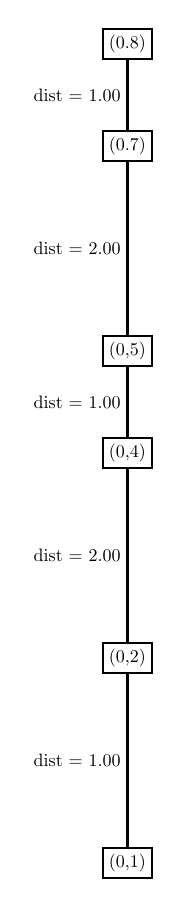
\begin{tikzpicture}[thick,scale=0.65, every node/.style={scale=0.65}]
    \begin{scope}
        \node[draw] (A) at (0,0) {(0,1)};
        \node[draw] (B) at (0,4) {(0,2)};
        \node[draw] (C) at (0,8) {(0,4)};
        \node[draw] (D) at (0,10) {(0,5)};
        \node[draw] (E) at (0,14) {(0.7)};
        \node[draw] (F) at (0,16) {(0.8)};
    \end{scope}

    \begin{scope}
        \draw (A) -- node[midway, left] {dist = 1.00} (B);
        \draw (B) -- node[midway, left] {dist = 2.00} (C);
        \draw (C) -- node[midway, left] {dist = 1.00} (D);
        \draw (D) -- node[midway, left] {dist = 2.00} (E);
        \draw (E) -- node[midway, left] {dist = 1.00} (F);
    \end{scope}
\end{tikzpicture}